\documentclass{article}
\setlength{\parskip}{5pt} % esp. entre parrafos
\setlength{\parindent}{0pt} % esp. al inicio de un parrafo
\usepackage{amsmath} % mates
\usepackage{listings}
\usepackage[sort&compress,numbers]{natbib} % referencias
\usepackage{url} % que las URLs se vean lindos
\usepackage[top=25mm,left=20mm,right=20mm,bottom=25mm]{geometry} % margenes
\usepackage{hyperref} % ligas de URLs
\usepackage{graphicx} % poner figuras
\usepackage[spanish]{babel} % otros idiomas
\usepackage{textcomp}
\usepackage{pgfplots} % crear graficas
\pgfplotsset{width=9cm,compat=1.7}
\title{"P1" Movimiento Browniano}
\author{NESTOR RODRIGUEZ}
\date{Febrero 2022}

\begin{document} % inicia contenido

\maketitle % cabecera
\section{Introducción}
\setlength{\parskip}
\setlength{\parindent}
\usepackage{El primer reto es estudiar de forma sistemática y automatizada el tiempo de ejecución de una caminata (en milisegundos) en términos del largo de la caminata (en pasos) y la dimensión. Para medir el tiempo de una réplica, ejecútala múltiples veces y normaliza con la cantidad de repeticiones para obtener un promedio del tiempo de una réplica individual.
El segundo reto es realizar una comparación entre una implementación paralela y otra versión que no aproveche paralelismo en términos del tiempo de ejecución, aplicando alguna prueba estadística adecuada para determinar si la diferencia es significativa.}

\begin{document} % inicia contenido

\maketitle % cabecera

\section{Objetivo}
El objetivo de esta práctica es examinar de manera sistemática los efectos de la dimensión en la distancia Euclideana máxima del origen del movimiento Browniano para dimensiones 1, 2, 3, 4 y 5, variando el número de pasos de la caminata (100, 1000 o 10000 pasos), con 30 repeticiones del experimento para cada combinación (1 con 100, 1 con 1000, 1 con 10000, 2 con 100, 2 con 1000, etc.) y graficar todos los resultados en una sola figura con diagramas de caja-bigote.

\section{Desarrollo} % seccion y etiqueta
La definicion de Movimiento Browniano: hace referencia al movimiento de partículas microscopicas que experimentan un movimiento aleatorio debido a fluctuaciones termicas, fenómeno observado por primera vez en 1827 por R. Brown y descrito formalmente en 1905 por A. Einstein.
Así que con esto se realizo para generar el código con objetivo de la práctica, esto se encuentran en: 
\href{https://https://github.com/NestorZeus/SIMULACION-COMPUTACIONAL-DE-NANOMATERIALES/blob/main/P1/Homework1.py}{mi repositorio}  en GitHub. Inicie tomando como base el Tomando como base la página \href{https://github.com/satuelisa/Simulation/blob/master/BrownianMotion/sinpar.py}{c\'odigo} proporcionado por la Dra. Elisa Schaeffer \cite{elisa1}, se hace una modificacion para iterar entre la cantidad de pasos que se realizan en cada dimension. 

\subsection {Ejecución en Python}
A continuacion se realiza el siguiente ejercicio en código Python para la realización de la ejecución en los siguientes comandos.
\begin{lstlisting}

from random import random, randint
from math import fabs, sqrt
import matplotlib.pyplot as plt
import numpy as np
from time import time

runs = 30 #replicas
caminatas = [100, 1000, 10000] #pasos
results = [] #almacena las dimensiones

for i in range(3): #itera la cantidad de pasos
    dur = caminatas[i]
    for dim in range(1, 6): #de una a cinco dimensiones
        mayores = []
        for rep in range(runs):#corre el experimento 30 veces en cada dimension
            before = time()*1000
            pos = [0] * dim
            mayor = 0
            for paso in range(dur):
                eje = randint(0, dim - 1)
                if pos[eje] > -100 and pos[eje] < 100:
                    if random() < 0.5:
                        pos[eje] += 1
                    else:
                        pos[eje] -= 1
                else:
                    if pos[eje] == -100:
                        pos[eje] += 1
                    if pos[eje] == 100:
                        pos[eje] -= 1
                mayor = max(mayor, sqrt(sum([p**2 for p in pos])))
            mayores.append(mayor)
            after = time()*1000
        results.append(mayores)
tiempo = after - before
print(tiempo)

#separar los resultados en tres grupos de caminatas
walks_1 = results[0:4]
walks_2 = results[4:8]
walks_3 = results[8:12]

#empezar a graficar

ticks = ['1', '2', '3', '4', '5']

#funcion definir los colores de cajas y bigotes
def set_box_color(bp, color):
    plt.setp(bp['boxes'], color='green')
    plt.setp(bp['whiskers'], color='gray')
    plt.setp(bp['caps'], color='red')
    plt.setp(bp['medians'], color='purple')

def box_plot(data, edge_color, fill_color):
    bp = ax.boxplot(data, patch_artist=True)
    
    for element in ['boxes', 'whiskers', 'fliers', 'means', 'medians', 'caps']:
        plt.setp(bp[element], color=edge_color)

    for patch in bp['boxes']:
        patch.set(facecolor=fill_color)

    for patch, color in zip(box['boxes'], colors):
        patch.set_facecolor(color)

        
plt.figure()

bpl = plt.boxplot(walks_1, positions=np.array(range(len(walks_1)))*6.0-1.0, sym='-1', widths=1.2)
bpc = plt.boxplot(walks_2, positions=np.array(range(len(walks_2)))*6.0, sym='-1', widths=1.2)
bpr = plt.boxplot(walks_3, positions=np.array(range(len(walks_3)))*6.0+1.0, sym='-1', widths=1.2)
set_box_color(bpl, '#67001f')
set_box_color(bpc, '#1a1a1a')
set_box_color(bpr, '#d6604d')


plt.xticks(range(0, len(ticks)*5, 5), ticks)
plt.ylim(0, len(ticks)*40)
plt.xlim(-3, len(ticks)*5)
plt.title('Distancia Manhattan')
plt.tight_layout()
plt.savefig('DistanciaMan.png')
plt.show()
\end{lstlisting}

\section{Resultados}

En esta seccion se muestra la grafica Manhattan en corelacion de dimensiones 1, 2, 3, 4 y 5, variando el número de pasos de la caminata (100, 1000 o 10000 pasos), con 30 repeticiones del experimento para cada combinación (1 con 100, 1 con 1000, 1 con 10000, 2 con 100, 2 con 1000, etc.).


\section{Mediciones y Gráfica}
\begin{figure}
    \centering
    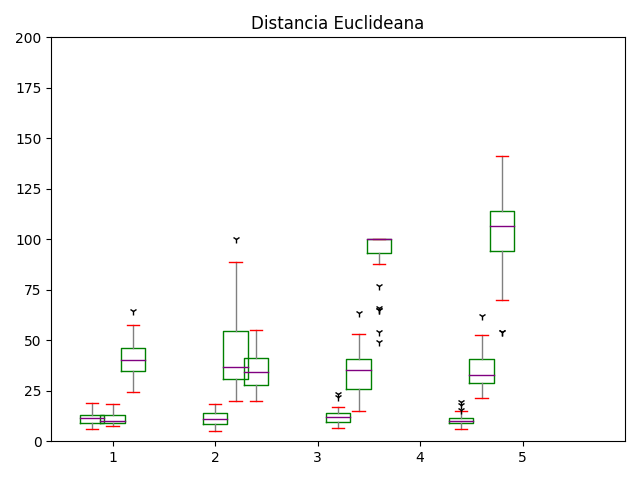
\includegraphics[width=150mm]{Figure_1.png}
    \caption{Diagrama caja-bigote en los grupos de 100, 1,000 y 10,000 pasos en dimensiones de 1 a 5 con 30 repeticiones.}
    \label{figure}
\end{figure}

Se observa la siguiente tabla en la distribucion de la medicion en los vectores en Python. A partir de las secciones anteriores encontramos que las principales características de este fenómeno son: Las partículas pequeñas tienen mayor velocidad. Las partículas se mueven más rápido en fluidos con poca viscosidad. La energía promedio de las partículas es proporcional a la temperatura. Aumenta la cantidad de pasos, lo cual se debe a que tiene las posibilidades de determinar en ciertos puntos diferentes del espacio.

\begin{table}[h!]
    \centering
    \caption{Mediciones para la distancia Euclideana máxima del origen del movimiento Browniano para dimensiones}
    \begin{tabular}{|r|r|r|r||r|r|r|r||r|r|r|r|}
    \hline
       Medición & Pasos  \\
       \hline\hline
        1, 2, 3,4 y 5 & 100 \\
        \hline
        1, 2, 3,4 y 5  & 1000 \\
        \hline
        1, 2, 3,4 y 5  & 10000 \\
        \hline

        
    \end{tabular}
    \label{medir_R}
\end{table}



\newpage
\section{Conclusion}

Se realizo la tarea 1 con éxito para obtener la caja-bigote para las repeticiones del experimento.
Al observar los diagramas de la figura \ref{figure} se caracteriza en que el rango del máximo que es amplio al aumentar la cantidad de pasos.


\bibliography{simulacion.bib}
\bibliographystyle{plain}

\end{document}
